% !TeX encoding = UTF-8
% !TeX spellcheck = en_GB
% !TeX root = ../thesis.tex

\chapter{Evaluation}\label{ch:evaluation}
Before any of the research questions could be answered, we searched for security patterns that are IoT-specific and already exist in literature. With the help of this newly created pattern catalogue we are now able to answer the previously stated RQs by following these steps:

\begin{enumerate}
	\item[RQ1] Compare the number of security patterns of each layer in the IoT WFRM.
	\item[RQ2] List the important security goals for an IoT system and check for each pattern which goals it protects. Compare the coverage of the different security goals.
	\item[RQ3] List the OWASP top ten most common security vulnerabilities within IoT and check if each vulnerability is solved by at least one pattern.
\end{enumerate}
	
	
\section{Data Set of IoT Security Primary Studies}\label{sec:patterns}
The foundation for the security pattern catalogue in Chapter~\ref{ch:catalogue}, which was created specifically for this master's thesis, can be found in Table~\ref{tab:paper-set}. This table showcases in chronological order the collected data set of primary studies that are focused on IoT security patterns.

\begin{longtable}[c]{llp{6.5cm}l}
	\caption{Overview of primary IoT security pattern studies}
	\label{tab:paper-set} \\
	\hline
	\textbf{Year} & \textbf{Author} & \textbf{Title} & \textbf{Paper \#} \\
	\hline
	\endfirsthead
	%
	\multicolumn{4}{c}%
	{{\bfseries Table \thetable\ continued from previous page}} \\
	\endhead
	%
	2021 & Fernández et al. & A Pattern for a Secure IoT Thing & \cite{Fernandez2021} \\
	2021 & Papoutsakis et al. & Towards a Collection of Security and Privacy Patterns & \cite{Papoutsakis2021} \\
	2020 & Fernández et al. & Abstract and IoT security segmentation patterns & \cite{Fernandez20201} \\
	2020 & Fernández et al. & Secure Distributed Publish/Subscribe (P/S) pattern for IoT & \cite{Fernandez20202} \\
	2020 & Fernández et al. & A Pattern for a Secure Cloud-Based IoT Architecture & \cite{Fernandez20203} \\
	2020 & Mu\~{n}oz et al. & TPM, a Pattern for an Architecture for Trusted Computing & \cite{Munoz2020} \\
	2020 & Orellana et al. & A Pattern for a Secure Sensor Node & \cite{Orellana2020} \\
	2019 & Moreno et al. & BlockBD: A Security Pattern to Incorporate Blockchain in Big Data Ecosystems & \cite{Moreno2019} \\
	2018 & Ali et al. & Applying security patterns for authorization of users in IoT based applications & \cite{Ali2018} \\
	2018 & Schu\ss{} et al. & IoT Device Security the Hard(Ware) Way & \cite{Schuss2018} \\
	2018 & Seitz et al. & Fogxy: An Architectural Pattern for Fog Computing & \cite{Seitz2018} \\
	2018 & Tkaczyk et al. & Cataloging design patterns for internet of things artifact integration & \cite{Tkaczyk2018} \\
	2017 & Lee et al. & A case study in applying security design patterns for IoT software system & \cite{Lee2017} \\
	2017 & Reinfurt et al. & Internet of Things Security Patterns & \cite{Reinfurt20172} \\
	2016 & Sinnhofer et al. & Patterns to Establish a Secure Communication Channel & \cite{Sinnhofer2016} \\
	2016 & Syed et al. & A Pattern for Fog Computing & \cite{Syed2016} \\
	2015 & Ur-Rehman et al. & Secure Design Patterns for Security in Smart Metering Systems & \cite{Ur-Rehman2015} \\
	2014 & Ciria et al. & The History–Based Authentication pattern & \cite{Ciria2014} \\
	2007 & Fernández et al. & Security Patterns for Physical Access Control Systems & \cite{Fernandez2007} \\
	2005 & Kienzle et al. & Security patterns repository, version 1.0 & \cite{Kienzle2006} \\
	\hline
\end{longtable}


\section{RQ1: IoT World Forum Reference Model Categorization}\label{sec:rq1}
In order to answer RQ1 \emph{\q{Which layer in the IoT WFRM is covered by the least security patterns?}}, we went through each paper in our data set in Table~\ref{tab:paper-set} and assigned each pattern to its corresponding layer in the model. The pattern distribution for each WFRM layer is illustrated with a corresponding pie chart in Figure~\ref{fig:rq1}.

\begin{figure}[ht]
	\centering
	\includegraphics[width=0.9\linewidth]{img/RQ1}
	\caption{The WFRM layer distribution of IoT security patterns}
	\label{fig:rq1}
\end{figure}

According to the calculated distribution of IoT security patterns that are attributed to the different layers of the WFRM, most patterns can be almost equally found in the Application (L5) and Connectivity (L2) layers. With 15 and 14 patterns respectively these two layers take almost half of the total of 61 IoT security patterns that were found during our search process. The Edge Computing (L3) and Data Accumulation (L4) layers on the other hand are with three patterns each on the lower end of the pattern coverage. When looking at the reasoning for this occurrence, we can say that Edge Computing can be seen as an own technology infrastructure that not all models consider a part of IoT. If we specifically searched for Edge functionality in publications, our success rate in finding such patterns would definitely be significantly higher. But because IoT was the main focus of our research topic, only a few publications that specified IoT as well as Edge technology at the same time could be found. The reason for Data Accumulation (L4) being under-represented with IoT security patterns in our study is definitely worth analysing further. Maybe because a secure storage is a big part of any computer system, mobile or stationary devices, there are only a few patterns that exist to date that specifically try to solve security problems in IoT devices. In conclusion, for a better distribution of patterns in the WFRM architecture the development of IoT security patterns for the Data Accumulation layer is encouraged.
 

\section{RQ2: Protected Security Goals}\label{sec:rq2}
With the second RQ we want to answer the question which security goals are covered by the patterns in the catalogue of Chapter~\ref{ch:catalogue} and how the coverage of the rest can be improved. Like for RQ1 we looked at each paper from the data set in Table~\ref{tab:paper-set} and assigned the specific security goals to each of them. The total number of times each security objective is covered by a pattern is shown in Table~\ref{tab:rq2}.

\begin{table}[ht]
	\centering
	\caption{Security objectives addressed by IoT security patterns}
	\label{tab:rq2}
	\begin{tabular}{l|c}
		\hline
		\textbf{Security Objective} & \textbf{Pattern Count} \\
		\hline
		Confidentiality     & 30    \\
		Integrity           & 20    \\
		Availability        & 18    \\
		Authentication      & 27    \\
		Authorization       & 24    \\
		\hline
	\end{tabular}
\end{table}

With a total of 30 publications the confidentiality objective is the goal that is covered the most in our data set. It is a security requirement that is surely easier to achieve than the others, because any system should protect their sensitive data. Thus, even if an IoT system is built without any security aspects in mind, the probability that confidentiality is ensured is pretty high. Therefore, it is usual that there exist many patterns that guarantee this objective. Availability, however, is the security goal with the least amount of coverage. The objective to ensure that a system is accessible for as long and often as possible can be quite challenging. One other reason for this could be, that when thinking about security, availability is not the most obvious choice compared to confidentiality or integrity. But by keeping the aspect of replication in mind to ensure availability when developing new IoT technologies, IoT architectures will be more secure in the future. 

\begin{figure}[ht]
	\centering
	\includegraphics[width=0.9\linewidth]{img/RQ2}
	\caption{IoT security patterns with their security concerns per WFRM layer}
	\label{fig:rq2}
\end{figure}

Figure~\ref{fig:rq2} compares the coverage of different security objectives in each layer of the WFRM architecture. The outlier in the bar plot is definitely the Data Accumulation (L4) layer. With only three security goals being covered and authentication and authorization being absent entirely, one sees clearly the lack of security solutions for storages of IoT devices. When analysed further one could say, that the reason for authentication being neglected lies in these mechanisms usually being implemented in higher layers of the IoT architecture. Interesting to mention is also the lack of availability support in the Collaboration \& Processes (L7) layer. But because this layer is focused on user interactions and not the applications of the system themselves, it makes sense that availability is not a priority here. 


\section{RQ3: Solutions for Common Vulnerabilities}\label{sec:rq3}
Looking at the OWASP top ten IoT vulnerabilities there are countless of new issues that arise every year while developing IoT systems. In RQ3 we now want to know if any of the security patterns in our pattern catalogue in Chapter~\ref{ch:catalogue} are able to solve some of these common mistakes developers tend to make in IoT environments. The following Figure~\ref{fig:rq3} shows which common vulnerabilities can be solved with the found IoT security patterns. 

\begin{figure}[ht]
	\centering
	\includegraphics[width=0.9\linewidth]{img/RQ3}
	\caption{Potential pattern solutions for the OWASP common vulnerabilities}
	\label{fig:rq3}
\end{figure}

It seems that each common vulnerability from the OWASP top ten can be (partially) solved by at least one IoT security pattern from our catalogue. The easiest one to fix is apparently T7 which focuses on insecure data transfer and storage. At least 34 different IoT security patterns that we found have a solution that could remove parts of the vulnerability and improve the handling of data in IoT devices. On the other hand T4 is apparently the hardest one to solve with only one pattern addressing this issue. If we look into its description, the problem is the lack of ability to securely update the IoT device. This is a very specific issue that also is highly dependent on the hardware of the device and its user interface. For a better update management of IoT devices further research in terms of security patterns is highly recommended in this area.

When we now look into the WFRM layer distribution of the IoT security patterns for each individual OWASP vulnerability, the pie charts in Figure~\ref{fig:pies} mirror the results of the previous bar plot. While the pie charts for T2, T3 and T7 (see Figures~\ref{fig:t2}, \ref{fig:t3}, and \ref{fig:t7} respectively) show the most diverse range of pattern solutions from up to six different layers, the one for T4 in Figure~\ref{fig:t4} has only patterns from the Physical Devices \& Controllers (L1) layer. 

\begin{figure}[ht]
	\centering
	\includegraphics[width=0.4\linewidth]{img/legend}
	\caption{Legend for pie charts}
	\label{fig:legend}
\end{figure}

\begin{figure}[ht]
	\centering
	\subfigure[][]{
		\label{fig:t1}
		\includegraphics[height=1in]{img/T1}}
	\subfigure[][]{
		\label{fig:t2}
		\includegraphics[height=1in]{img/T2}}
	\subfigure[][]{
		\label{fig:t3}
		\includegraphics[height=1in]{img/T3}}
	\subfigure[][]{
		\label{fig:t4}
		\includegraphics[height=1in]{img/T4}}
	\subfigure[][]{
		\label{fig:t5}
		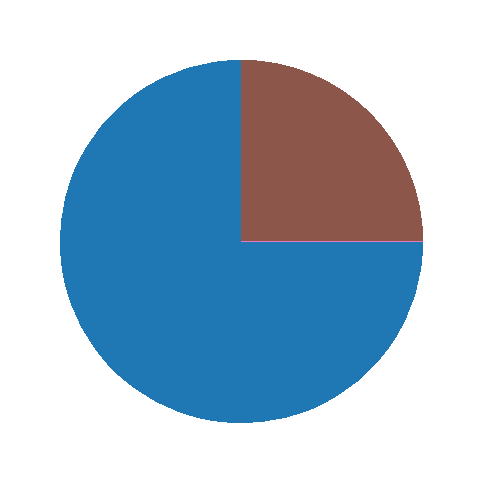
\includegraphics[height=1in]{img/T5}} \\
	\subfigure[][]{
		\label{fig:t6}
		\includegraphics[height=1in]{img/T6}}
	\subfigure[][]{
		\label{fig:t7}
		\includegraphics[height=1in]{img/T7}}
	\subfigure[][]{
		\label{fig:t8}
		\includegraphics[height=1in]{img/T8}}
	\subfigure[][]{
		\label{fig:t9}
		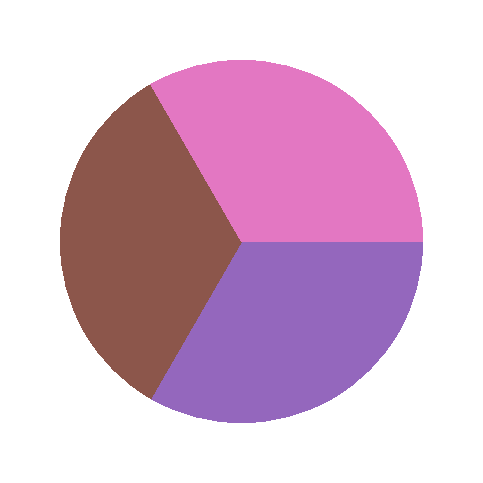
\includegraphics[height=1in]{img/T9}}
	\subfigure[][]{
		\label{fig:t10}
		\includegraphics[height=1in]{img/T10}}
	\caption[Layer distribution of pattern solutions for OWASP top ten]{Layer distribution of security patterns that address the OWASP top ten with one pie chart per vulnerability: 
		\subref{fig:t1} T1;
		\subref{fig:t2} T2;
		\subref{fig:t3} T3; 
		\subref{fig:t4} T4; 
		\subref{fig:t5} T5; 
		\subref{fig:t6} T6; 
		\subref{fig:t7} T7;
		\subref{fig:t8} T8;  
		\subref{fig:t9} T9; and
		\subref{fig:t10} T10.}
	\label{fig:pies}
\end{figure}

Therefore, we see a connection between the found IoT security patterns for a specific OWASP vulnerability and the number of layers the various solutions are from. This assumption is confirmed by the following Figure~\ref{fig:corr}, which consists of a scatter plot that showcases the correlation between the pattern quantity and their layer distribution with a value of 0.86808368. This correlation coefficient always ranges from -1 to 1 and indicates the strength of the relationship between two variables. A value between 0.7 and 1 shows a strong connection and the positive sign indicates, that more patterns as solutions for a specific vulnerability also mean a more diverse distribution of WFRM layers for these IoT patterns. 

\begin{figure}[ht]
	\centering
	\includegraphics[width=0.9\linewidth]{img/correlation}
	\caption{The correlation between the number of patterns and WFRM layers for each OWASP vulnerability.}
	\label{fig:corr}
\end{figure}


\section{Use Case Application}\label{sec:use_case}
Before we discuss the findings of our research work, let's see how the created pattern catalogue can be used in a real life situation. The pattern collection was designed to easily function as a checklist. To showcase the pattern selection process, we describe the following IoT home scenario. It is important to note, that in this example we assume that the system is only used by the owner of the house and no further security measures were taken than the ones that were already integrated into the system. 

This smart home contains different connected devices that are distributed in the living room, bedroom, kitchen, bathroom and entrance of the house. All electronic devices run on the custom firmware Tasmota\footnote{\href{https://tasmota.github.io/docs}{https://tasmota.github.io/docs, last accessed: 25.02.2023.}} and include: Four RGB LED  bulbs\footnote{\href{https://www.tasmota.shop/gb/lights/7-led-rgb-bulb-wifi-e27-15w.html}{https://www.tasmota.shop/gb/lights/7-led-rgb-bulb-wifi-e27-15w.html, last accessed: 25.02.2023.}}, six Shelly\footnote{\href{https://www.shelly.cloud/en-de/products/product-overview/1xs1}{https://www.shelly.cloud/en-de/products/product-overview/1xs1, last accessed: 25.02.2023.}} that function as light controllers, and five smart plugs\footnote{\href{https://www.amazon.de/dp/B07D73S72W}{https://www.amazon.de/dp/B07D73S72W, last accessed: 25.02.2023.}}. In addition, a Raspberry PI with HomeBridge\footnote{\href{https://homebridge.io}{https://homebridge.io, last accessed: 25.02.2023.}} allows the integration of HomeKit into the network that controls the following devices: Two televisions\footnote{\href{https://plugins.hoobs.org/plugin/homebridge-samsung-tizen}{https://plugins.hoobs.org/plugin/homebridge-samsung-tizen, last accessed: 25.02.2023.}}, four Sonos ZonePlayers\footnote{\href{https://plugins.hoobs.org/plugin/homebridge-zp}{https://plugins.hoobs.org/plugin/homebridge-zp, last accessed: 25.02.2023.}}, a Ring camera and doorbell\footnote{\href{https://plugins.hoobs.org/plugin/homebridge-ring}{https://plugins.hoobs.org/plugin/homebridge-ring, last accessed: 25.02.2023.}}.

After we established the use case example, we can inspect each pattern of the catalogue in Chapter~\ref{ch:catalogue} and check its applicability in the given context. The evaluation results can be found in Table~\ref{tab:use-case} with (-) indicating this pattern is not suitable for this system, (o) being used in cases where the given system has already implemented similar security features this pattern would provide, and (+) marking recommended patterns to implement to further optimize the system design.  

\begin{landscape}
\begin{longtable}[c]{llcp{12cm}}
	\caption{Use case applicability of patterns}
	\label{tab:use-case} \\
	\hline
	\textbf{\#} & \textbf{Pattern} & \textbf{Rating} &
	\textbf{Explanation} \\
	\hline
	\endhead
	%
	\ref{p:hardware} & Hardware IoT Security & + & Exchangeable cryptographic co-processors to secure IoT devices. \\
	\ref{p:thing} & Secure IoT Thing & + & Secure any entity that is connected to sensors/actuators, e.g Raspberry PI. \\
	\ref{p:node} & Secure Sensor Node & - & System does not include sensor nodes. \\
	\ref{p:segment} & Security Segmentation & + & IoT devices are divided into subnetworks. \\
	\ref{p:tpm} & Trusted Platform Module & + & Attestation of Raspberry PI with integrated cryptographic services. \\
	\hline
	\ref{p:ac} & Authenticated Channel & o & Mutual authentication of communication partners and forward secrecy. \\
	\ref{p:ec} & Encrypted Channel & o & TLS handshake and exchange of cryptographic information. \\
	\ref{p:broker} & Middleware Message Broker & o & HomeBridge controls the flow of messages between IoT devices. \\
	\ref{p:scmessage} & Middleware Self-contained Message & + & Messages should be \q{pure and complete} representations of events/commands. \\
	\ref{p:sdn} & Orchestration of SDN Network Elements & - & Only required when an IoT SDN is employed. \\
	\ref{p:con} & Outbound-Only Connection & + & Blocks incoming malicious connection requests. \\
	\ref{p:keyex} & Password Based Key Exchange & + & Common secret is used to generate session key pairs. \\
	\ref{p:sc} & Safe Channel & o & Use certificates to guarantee integrity during message transmission. \\
	\ref{p:readout} & Secure Remote Readout & + & Security Module encrypts measurements before transmitting. \\
	\ref{p:sm} & Signed Message & o & Use digital signatures during the message generation/exchange process. \\
	\ref{p:crypto} & Symmetric Key Cryptography & + & Handshake and common secret are exchanged between communication parties. \\
	\ref{p:auc} & Third Party Based Authentication & + & Combination of asymmetric cryptography and session keys. \\
	\ref{p:partner} & Trusted Communication Partner & + & List trusted communication partners and block unknown connection requests. \\
	\ref{p:trust} & Web of Trust & - & Tasmota uses a central self-signed certificate authority. \\
	\hline
	\ref{p:fog} & Fog Computing & - & No cloud-based system. \\
	\ref{p:fogxy} & Fogxy & - & No cloud-based system. \\
	\ref{p:cloud} & Secure Cloud-based IoT Architecture & - & No cloud-based system. \\
	\hline
	\ref{p:es} & Encrypted Storage & + & Critical data is encrypted before it gets committed to disk. \\
	\ref{p:rs} & Redundant Storage & - & No cloud-based system. \\
	\ref{p:ss} & Safe Storage & + & Guarantee integrity of stored data. \\
	\hline
	\ref{p:translation} & Alignment-based Translation Pattern & o & HomeBridge enables interoperability between different platforms. \\
	\ref{p:block} & BlockBD & - & No Big Data system. \\
	\ref{p:discover} & Discovery of IoT Services & - & No usage of different IoT services. \\
	\ref{p:flow} & Flow-based Service Composition & - & No usage of different IoT services. \\
	\ref{p:gateway} & IoT Gateway Event Subscription & o & HomeBridge sends notifications on updates. \\
	\hline
	\ref{p:ssl} & IoT SSL Cross-Layer Secure Access & o & Only authenticated entities are able to access the external interfaces. \\
	\ref{p:msgtranslator} & Middleware Message Translator & o & HomeBridge enables interoperability between different platforms. \\
	\ref{p:middleware} & Middleware Simple Component & + & Universally applicable pattern to achieve the best component decomposition. \\
	\ref{p:rest} & REST Request/Response & o & HomeBridge API is used to connect to different IoT devices. \\
	\ref{p:sandbox} & Server Sandbox & + & Isolate server to protect it in case the system gets compromised. \\
	\ref{p:orchest} & Service Orchestration & - & No usage of different IoT services. \\
	\ref{p:ontology} & Translation with Central Ontology & o & HomeBridge enables interoperability between different platforms. \\
	\hline
	\ref{p:acp} & Access Control to Physical Structures & - & No physical structures need to be accessed. \\
	\ref{p:alarm} & Alarm Monitoring & o & Alarm functionality is included in HomeBridge. \\
	\ref{p:log} & Audit Log & o & HomeBridge has a rolling log screen. \\
	\ref{p:acs} & Authenticated Session & - & System runs on a local server with no internet requirements. \\
	\ref{p:aze} & Authorization Enforcer & - & Only relevant if system is used by users with different roles. \\
	\ref{p:ep} & Encrypted Processing & + & Integrity of data with e.g homomorphic functions or secure multi-party computation. \\
	\ref{p:fault} & Fault Management & + & Smart handling of any faulty behaviour of the system. \\
	\ref{p:fac} & File Authentication & - & Only relevant if system is used by users with different privileges. \\
	\ref{p:mac} & Matrix Authentication & - & Only relevant if system is used by users with different privileges. \\	
	\ref{p:mine} & Minefield & + & Modify Raspberry PI to confuse attackers and simplify threat detection. \\
	\ref{p:rac} & Remote Authenticator/Authorizer & - & System runs on a local server with no internet requirements. \\
	\ref{p:rbac} & Role Based Access Control & - & Only relevant if system is used by users with different roles. \\
	\ref{p:sp} & Safe Processing & + & Guarantee integrity during data processing with e.g integrity checks. \\
	\ref{p:sdps} & Secure Distributed Publish/Subscribe & o & HomeBridge sends notifications on updates. \\
	\ref{p:uptime} & Uptime & o & HomeBridge measures and displays the server availability. \\
	\hline
	\ref{p:lockout} & Account Lockout & o & Login via password authentication. \\
	\ref{p:ace} & Authentication Enforcer & + & Authentication process that creates a proof of identity. \\
	\ref{p:black} & Blacklist & + & Identification of abusers who are not granted access to the system. \\
	\ref{p:hauc} & History-Based Authentication & + & Authentication is based on the user's own history. \\	
	\ref{p:control} & Permission Control & + & User can control which data is shared with the server. \\
	\ref{p:hub} & Personal Zone Hub & - & No cloud-based system. \\
	\ref{p:relays} & Relays & - & No switches in the system. \\
	\hline
	\ref{p:sap} & Single Access Point & + & Only one entry point into the system with HomeBridge UI. \\
	\ref{p:white} & Whitelist & + & Identification of trusted communication partners. \\
	\hline
\end{longtable}
\end{landscape}

While there are many patterns that are not suitable to be implemented in this kind of smart home scenario, like BlockBD~\ref{p:block} or the Web of Trust~\ref{p:trust}, just as many are already integrated into the system, e.g Uptime~\ref{p:uptime} or Account Lockout~\ref{p:lockout}. Nevertheless by going through the catalogue and analysing each pattern individually, we found 25 patterns that can be used to optimize the security measures in this smart home example. Spread across all layers of the WFRM architecture, one can choose from a variety of patterns that include Symmetric Key Cryptography~\ref{p:hardware}, Server Sandbox~\ref{p:sandbox} or even simpler solutions like a combination of a Blacklist~\ref{p:black} and a Whitelist~\ref{p:white}. 

This use case demonstrates that our pattern catalogue can act as an easy guideline to improve the security of a system. The evaluation process can be as straightforward as using the catalogue as a checklist while other approaches could include the sorting by WFRM layers or even by security objectives. Regardless of which method one uses, every system has vulnerabilities that can benefit from even the most obvious or trivial security features, like a Single Access Point~\ref{p:sap}.



 

